\subsection{Dresda coils}
The technology the HZDR team used to produce their coil is based on \textbf{circuit inkjet printing}.
Circuit inkjet printing consists of using a printer to \textbf{deposit conductive ink} on a substrate.
In this application, they used a \textbf{flexible substrate} to print the coil to allow it to be bent.

\begin{samepage}
    After printing the conductive ink is \textbf{tinned} to improve the conductivity of the coil and allow it to be soldered to other components.
    \nopagebreak

    \begin{figure}[H]
        \centering
        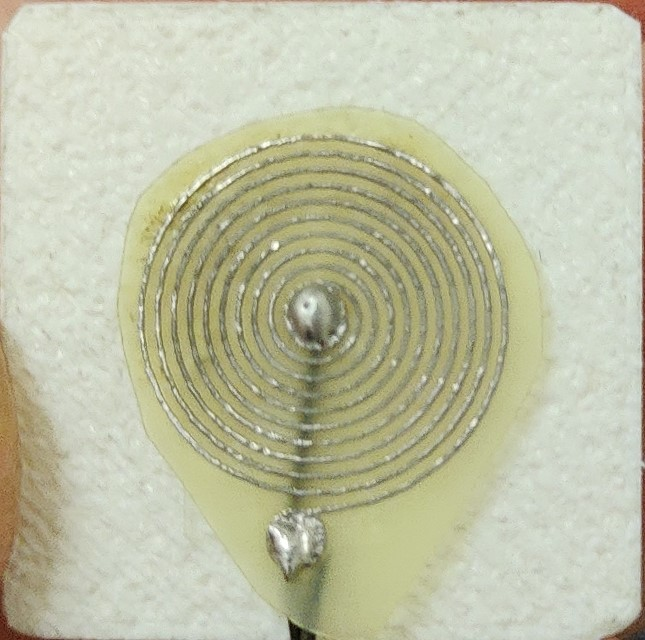
\includegraphics[width=0.4\linewidth]{Chapters/Chapter5/Coils_alternatives/Figures/Dresden_coil.jpg}
        \caption{Dresden coil \cite{HZDR}}
        \label{fig: Dresden_coil} 
    \end{figure}
\end{samepage}


\subsubsection{Low resistance and high power needs}
The Dresden coils have a resistance of about \textbf{2$\Omega$}, the external radius of \textbf{5e-3m}, the internal one of \textbf{0.84*e-3m}, and the number of spires equal to \textbf{11}.
We also know from the HZDR test that the coil can handle up to about \textbf{500mA} before starting to release too much heat.
This means a power limit of about \textbf{0.5W} for the coil.

\begin{samepage}
    The current limit is due to the \textbf{very low resistance} of the coil as for low applied voltages the coil will produce a lot of heat due to the \textbf{Joule effect} \ref{subsubsec: Joule_effect}.

    \begin{figure}[H]
        \centering
        \resizebox{0.5\textwidth}{!}{\begin{tikzpicture}
    \begin{axis}[
            xmin=0, ymin=0, xmax=3, ymax=2.5, samples=500,
            xlabel={Voltage [$V_{rms}$]},ylabel={Power [$W$]}, title={Power output vs $V_{rms}$}
        ]

        \addplot[blue, thick, domain=0:8, name path=func] (x, x^2/2);
        \addplot[red, thick, name path=limit] coordinates {
            (sqrt(0.5*2), \pgfkeysvalueof{/pgfplots/ymin}) 
            (sqrt(0.5*2), \pgfkeysvalueof{/pgfplots/ymax})
        }; % vertical limit line 

        \path[name path=axis] (axis cs:\pgfkeysvalueof{/pgfplots/xmin},0) -- (axis cs:\pgfkeysvalueof{/pgfplots/xmax},0);
        \path[name path=vend] (axis cs:\pgfkeysvalueof{/pgfplots/xmax},\pgfkeysvalueof{/pgfplots/ymin}) -- (axis cs:\pgfkeysvalueof{/pgfplots/xmax},\pgfkeysvalueof{/pgfplots/ymax});

        \addplot[red!25] fill between [of = limit and vend];
        % TODO: Add label to the limit line and legend
    \end{axis}
\end{tikzpicture}}
        \caption{Power profile of the Dresden coil}
        \label{fig: Dresden_heat_graph}
    \end{figure}
    As we can see in figure \ref{fig: Dresden_heat_graph}, after 1V the power limit is already reached.
\end{samepage}


\subsubsection{Low magnetic field strength}
For the same reason as the power limit, the magnetic field produced by the Dresden coil is \textbf{very low}.
Using the equation \ref{eq: Spiral_magn_field_eq} we can calculate the magnetic field produced by the Dresden coil on its surface and plot it as a function of the voltage applied to the coil (Fig. \ref{fig: Dresden_magnetic_field}).
\begin{figure}[H]
    \centering
    \resizebox{0.5\textwidth}{!}{\begin{tikzpicture}
    \begin{axis}[
            xmin=0, ymin=0, xmax=1, ymax=8e-3, samples=500,
            xlabel={Power [$P_{rms}$]},ylabel={Magnetic Field [$T$]}, title={Magnetic Field vs $P_{rms}$}
        ]

        \addplot[blue, thick, domain=0:3.5, name path=func] (x, 0.0021*x^0.5);
        \addplot[red, thick, name path=limit] coordinates {
            (0.5, \pgfkeysvalueof{/pgfplots/ymin}) 
            (0.5, \pgfkeysvalueof{/pgfplots/ymax})
        }; % vertical limit line 

        \path[name path=axis] (axis cs:\pgfkeysvalueof{/pgfplots/xmin},0) -- (axis cs:\pgfkeysvalueof{/pgfplots/xmax},0);
        \path[name path=vend] (axis cs:\pgfkeysvalueof{/pgfplots/xmax},\pgfkeysvalueof{/pgfplots/ymin}) -- (axis cs:\pgfkeysvalueof{/pgfplots/xmax},\pgfkeysvalueof{/pgfplots/ymax});

        \addplot[red!25] fill between [of = limit and vend];
        % TODO: Add label to the limit line and legend
    \end{axis}
\end{tikzpicture}}
    \caption{Magnetic field produced by the Dresden coil}
    \label{fig: Dresden_magnetic_field}
\end{figure}

As we can see in figure \ref{fig: Dresden_magnetic_field}, even at the power limit, the magnetic field produced by the Dresden coil is very low (in the order of 1mT).

\subsubsection{Fragility and low flexibility}
The Dresden coil is produced by using \textbf{three layers} of different materials.
The first layer is the substrate, which is made of a material similar to \textbf{paper}, the second layer is the \textbf{conductive ink}, and the third layer is the \textbf{tinning}.
The substrate is \textbf{not very flexible}, and neither is the tinning;
this makes the spires of the coil \textbf{easily damageable if bent repeatedly}.
Also, the tinning gets \textbf{cracked} by repeatedly heating and cooling the coil, which constantly happens during the coil's use.
The tinning cracking would happen multiple times during our tests, and we would have to \textbf{re-tin the damaged parts} of the coil to keep using it.